\input{head.tex}
\usepackage[printonlyused,nohyperlinks]{acronym}
\begin{document}
% \linenumbers
%\raggedright

\newcounter{myboxcounter}
\newcommand{\boxlabel}[1]{%
  \refstepcounter{myboxcounter}%
  \label{#1}%
}

\title{Supplemental: Application of qualifying variants for genomic analysis}

% target: Bioinformatics https://academic.oup.com/bioinformatics/

\author[1]{Dylan Lawless\thanks{Addresses for correspondence: \href{mailto:Dylan.Lawless@uzh.ch}{Dylan.Lawless@kispi.uzh.ch}}}
\author[2]{Ali Saadat}
\author[2]{Mariam Ait Oumelloul}
\author[2]{Simon Boutry}
\author[1]{Veronika Stadler}
\author[3]{Sabine Österle}
\author[3]{Jan Armida}
\author[4]{David Haerry}
\author[5]{D. Sean Froese}
\author[1]{Luregn J. Schlapbach}
\author[2]{Jacques Fellay}
%\author[1]{Consortium Members}
\affil[1]{Department of Intensive Care and Neonatology, University Children's Hospital Zürich, University of Zürich, Switzerland.}
\affil[2]{Global Health Institute, School of Life Sciences, École Polytechnique Fédérale de Lausanne, Switzerland.}
\affil[3]{SPHN Data Coordination Center, SIB Swiss Institute of Bioinformatics, Basel, Switzerland.}
\affil[4]{Positive Council, Zürich, Switzerland.}
\affil[5]{Division of Metabolism and Children’s Research Center, University Children’s Hospital Zürich, University of Zurich, Zurich, Switzerland.}

\maketitle
\justify
% \tableofcontents
% \listoffigures
% \listoftables



\clearpage
%\\\\\\\\\\\\\\\\\\\\\\\\\\\\
\beginsupplement
\section{Supplemental} \label{Supplemental_text}
\textbf{Application of qualifying variants for genomic analysis.}

\subsection{Validation study figures}

\begin{figure}[h]
\centering
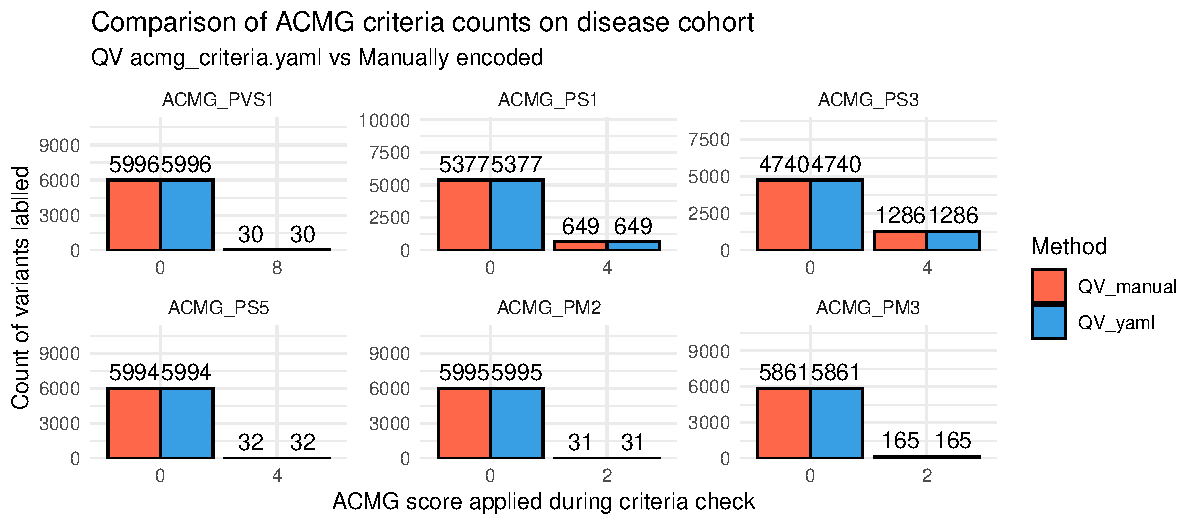
\includegraphics[width=0.9\textwidth]{./images/Guru_singlecase_validation_of_yaml_vs_manual.pdf}
\caption{Validation case study of a rare disease cohort of 940 WES individuals using an \ac{acmg} criteria subset, demonstrating a 100\% match between manually encoded and standalone YAML-based \ac{qv} for assigning pathogenicity scores.}
\label{fig:guru_singlecase_validation_of_yaml_vs_manual}
\end{figure}


\begin{figure}[h]
\centering
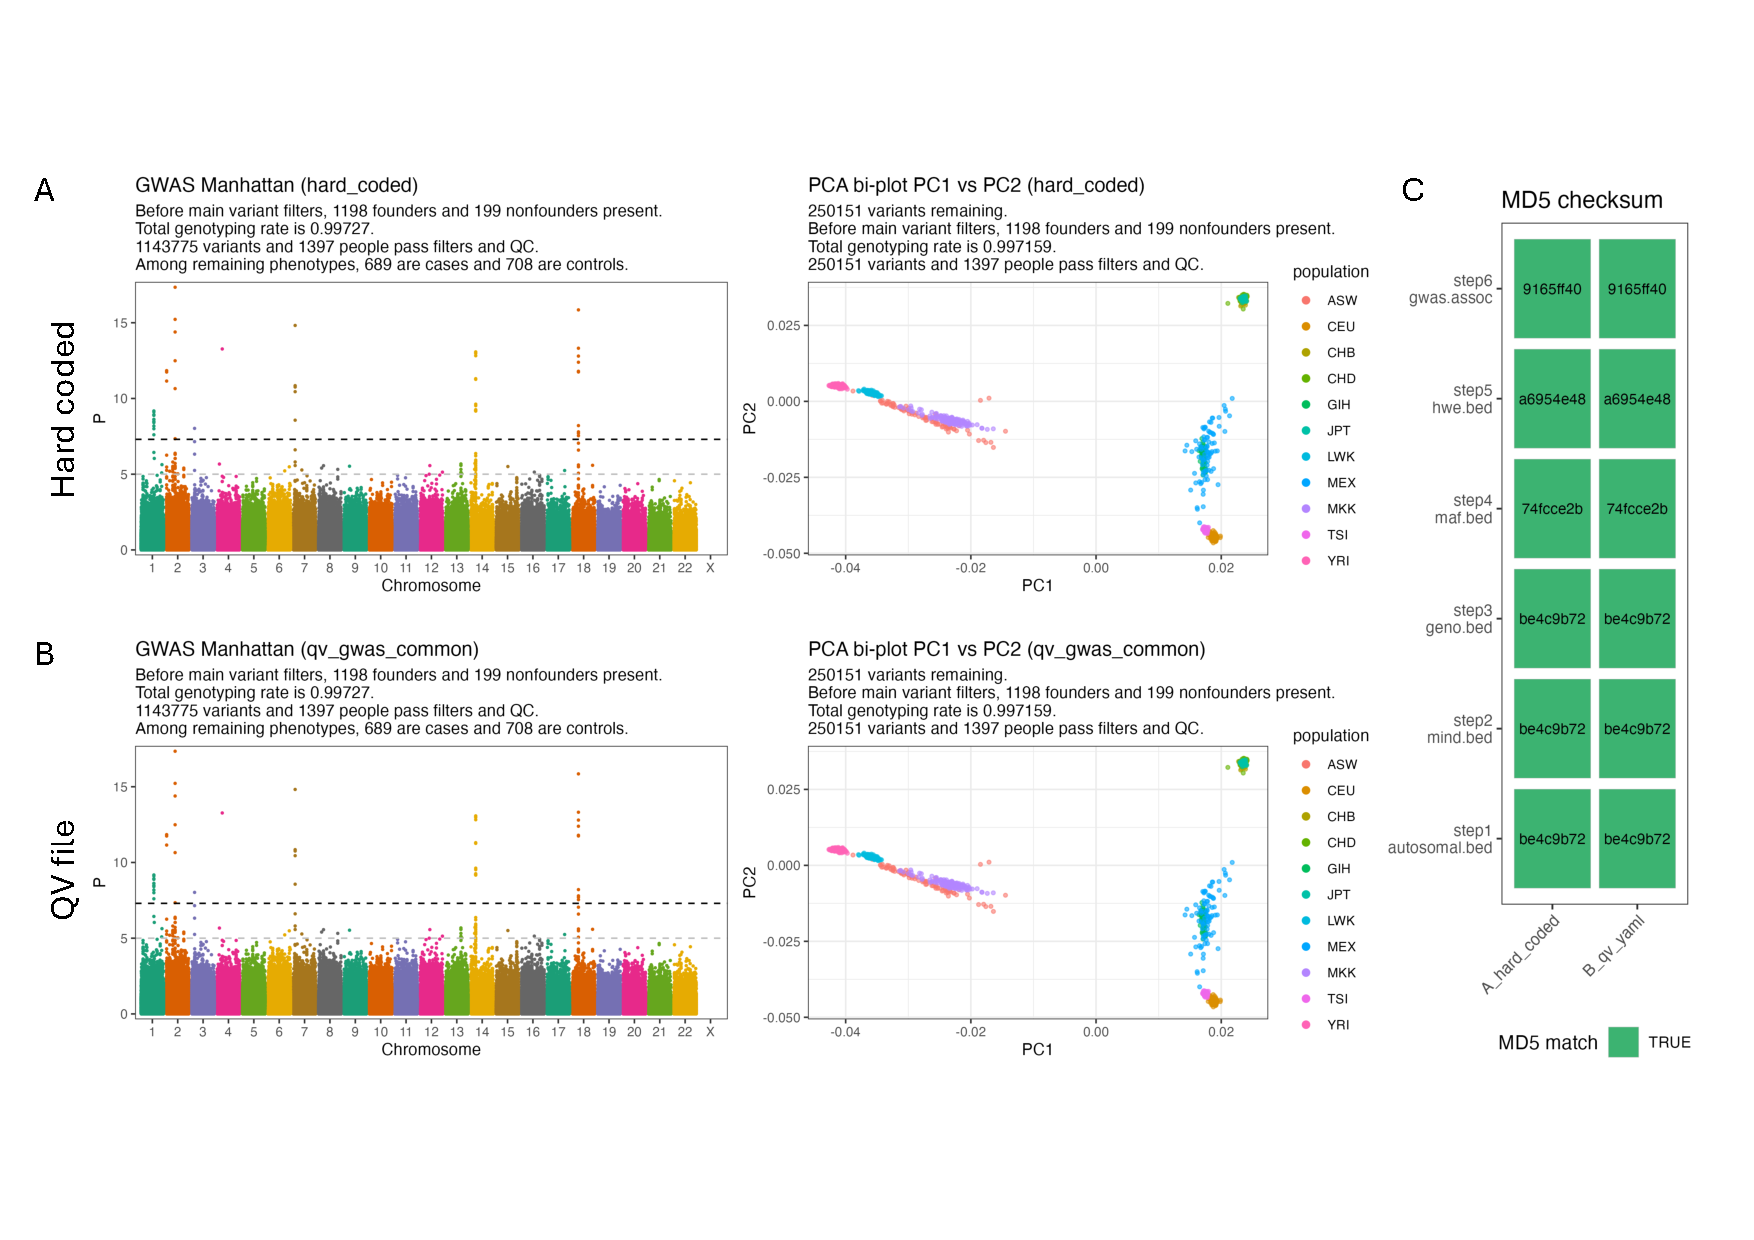
\includegraphics[width=\textwidth]{./images/hapmap_gwas_validation.pdf}
\caption{Validation in GWAS using QV parameterisation. 
(A) \ac{gwas} of simulated binary phenotypes in HapMap3 Phase 3 (R3) using a traditional variable embedded pipeline. Shown are the Manhattan plot of logistic regression results (left) and correction for population structure with principal component analysis (PC1 vs PC2, right). 
(B) Identical \ac{gwas} using a \ac{qv} YAML configuration file. The Manhattan and PCA results are indistinguishable from panel~A. 
(C) Verification of reproducibility. MD5 checksums of the main PLINK outputs are identical between panels~A and~B. The steps included processing of autosomal biallelic SNPs, sample call rate, variant call rate, minor allele frequency, Hardy–Weinberg equilibrium, and association results. The QV file encoded these thresholds (sample call rate $\geq$95\%, variant call rate $\geq$95\%, MAF $\geq$1\%, HWE p~$\geq$1e-6, autosomal biallelic SNPs only) together with covariates (sex and PC1-PC10) and logistic regression settings. This confirms that a shareable QV file reproduces hard-coded pipelines exactly while improving transparency and reusability.
}
    \label{fig:hapmap_gwas_validation}
\end{figure}

\begin{figure}[h]
\centering
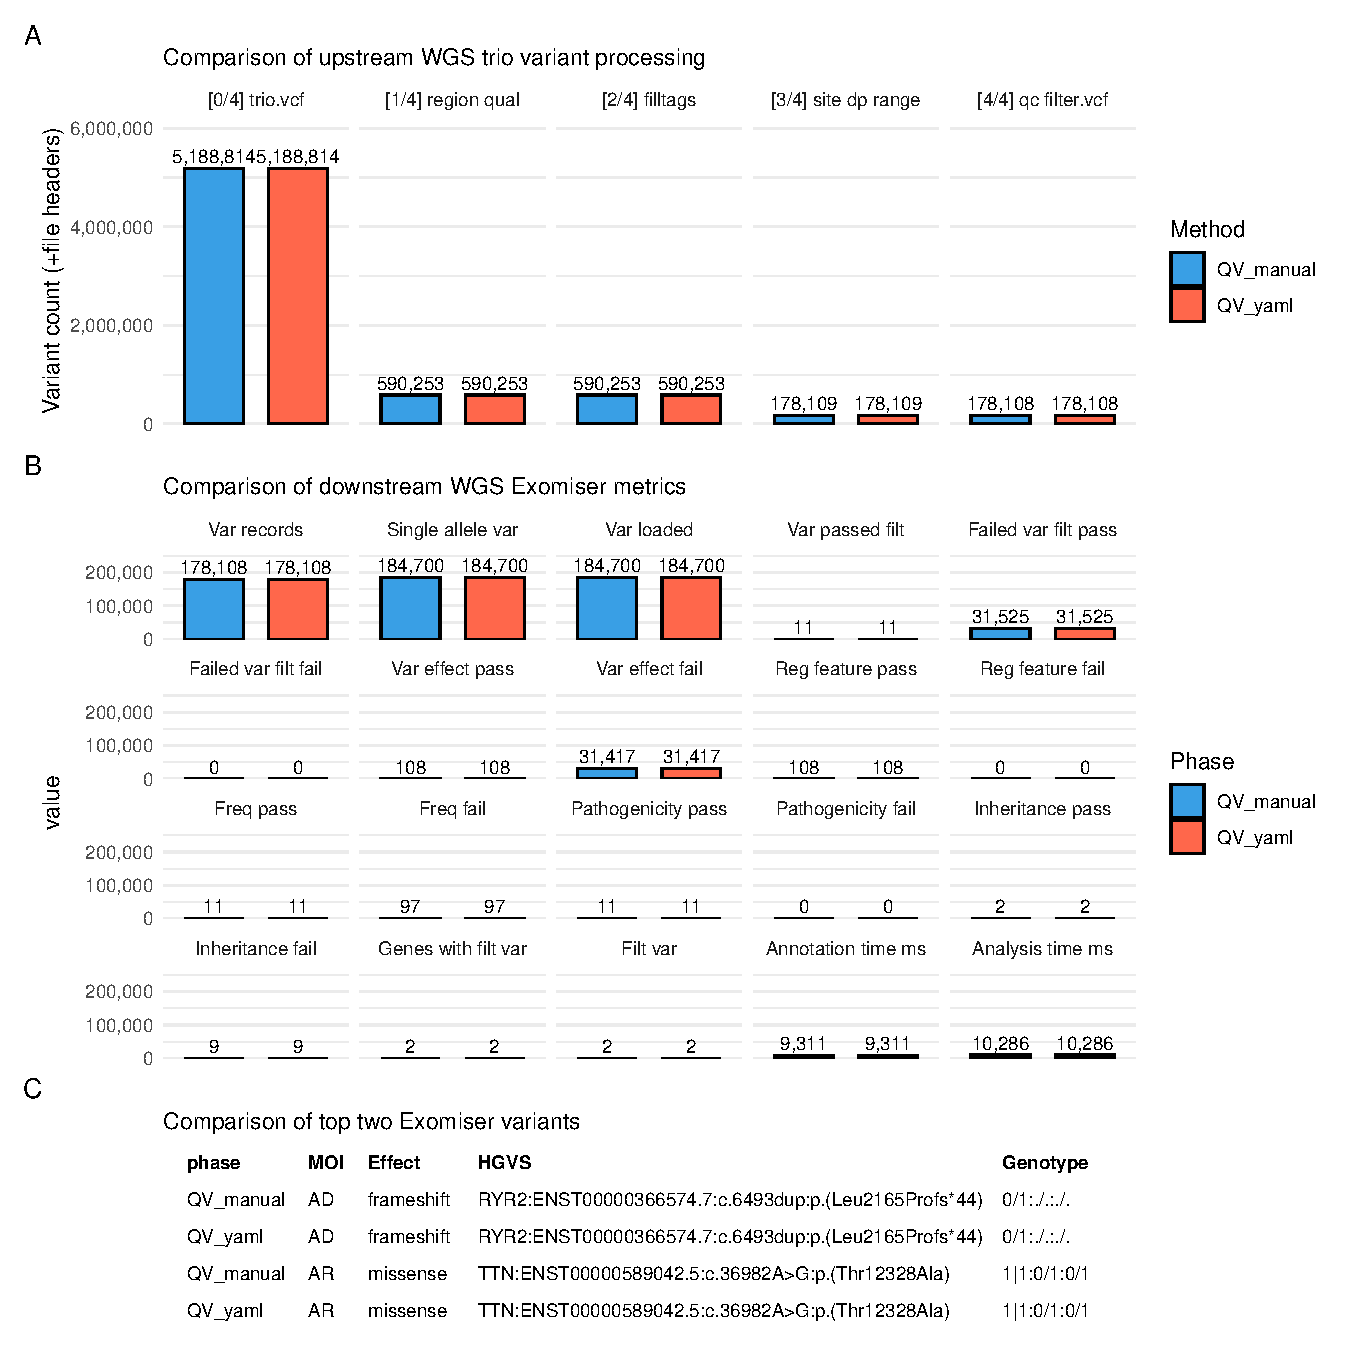
\includegraphics[width=\textwidth]{./images/qv_exomiser/exomiser_validation_bars_facet_metric.pdf}
\caption{Validation of the trio Exomiser pipeline using \ac{qv} parameterisation. 
\textbf{(A)} summarises upstream processing counts by file, 
\textbf{(B)} compares downstream Exomiser metrics, 
and \textbf{(C)} shows the key variant fields for the two variants identified. 
Variant counts in all panels confirm that intermediate files and final outputs are identical between configurations. 
The five preprocessing stages shown in~(A) are: 
(0) input trio VCF, (1) gene panel region and quality filtering, (2) tag annotation, (3) site-level depth range filtering, and (4) final QC-filtered VCF. 
MOI, mode of inheritance; HGVS, Human Genome Variation Society nomenclature.}
\label{fig:qv_exomiser_validation}
\end{figure}

\FloatBarrier
\subsection{Computational benchmark}\label{sec:benchmark}
Runtime performance was equivalent between traditional and \ac{qv}-based pipelines, as both read identical parameters from different sources. In the WGS trio validation study, pre-processing steps including filtering, \ac{qc}, and gene panel selection completed in 16–17~seconds, with a median difference of \textasciitilde0.5~seconds favouring the \ac{qv} YAML pipeline (\textbf{Figure \ref{fig:benchmark_preprocess_time_bars_by_step_elapsed}}). An incidental one-off 5~second delay arose from Singularity initialisation for the \texttt{yq} utility (step~0), a system-specific effect on our HPC and unrelated to the framework itself.

\begin{figure}[h]
\centering
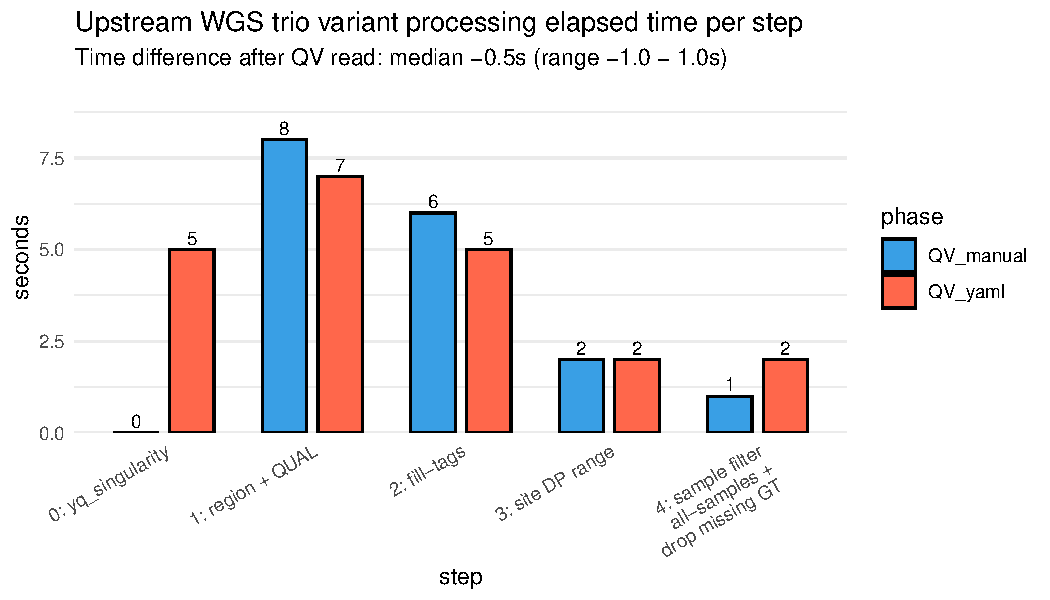
\includegraphics[width=\textwidth]{./images/qv_exomiser/benchmark_preprocess_time_bars_by_step_elapsed.pdf}
\caption{Benchmark of upstream preprocessing times in the WGS trio pipeline comparing \ac{qv}-based and traditional (manually parameterised) configurations. Stepwise elapsed times were nearly identical across both methods (median difference \textasciitilde0.5~s), with a fixed 5~s overhead from optional Singularity initialisation of \texttt{yq} in the \ac{qv} pipeline. The four preprocessing steps correspond to: (1) gene panel region and quality filtering of the trio VCF, (2) annotation of variant tags, (3) site-level depth range filtering, and (4) per-sample genotype filtering and exclusion of missing genotypes. All steps used \texttt{BCFtools} on VCF preprocessing, as illustrated in \textbf{Figure~\ref{fig:qv_exomiser_validation} (A)}.}
\label{fig:benchmark_preprocess_time_bars_by_step_elapsed}
\end{figure}



\subsection{How to build a QV file}

We recommend YAML or JSON for portability and adoption. You can build a QV in three ways:

\subsubsection*{Option 1: use the HTML QV builder (Zenodo)}
\begin{enumerate}
\item Open the HTML builder from the Zenodo repository.
\item Enter simple \texttt{key=value} statements in the left pane.
\item Copy or download the generated YAML.
\end{enumerate}

\noindent Example input lines:
\begin{verbatim}
meta qv_set_id="qv_gwas_common_v1_20250827"
meta version="1.0.0"
meta title="GWAS common QC"
meta authors=Alice,Bob
meta tags=GWAS,QC,PCA
filter maf_minimum field=MAF operator=">=" value=0.01 desc="Minimum MAF"
filter hwe field=HWE_P operator=">=" value=1e-6 logic=keep_if
filter region_include desc="include panel" field=OVERLAP(targets.exome.bed) 
    >>>> operator=">=" value=1 logic=keep_if
criteria disease_panel logic=and desc="HIGH impact within panel"
criteria disease_panel field=IMPACT operator="==" value=HIGH
criteria disease_panel field=OVERLAP(targets.exome.bed) operator=">=" value=1
meta description_patient=
    >>>> "There is a strong family history of early heart attacks."
meta description_ppie=
    >>>> "The PPIE group reviewed and approved the criteria on 2025-08-15."
\end{verbatim}

\subsubsection*{Option 2: write YAML by hand}
Minimal pattern:
\begin{verbatim}
meta:
  qv_set_id: qv_disease_panel_v1_20250828
  version: 1.0.0
  title: Disease panel filter
filters:
  region_include:
    description: Restrict to curated disease gene panel
    logic: keep_if
    field: OVERLAP(targets.disease_panel.bed)
    operator: ">="
    value: 1
criteria:
  pathogenic:
    description: Variant classified as pathogenic or likely pathogenic
    logic: and
    conditions:
      - group: any_of:start
      - { field: CLASS, operator: "==", value: P }
      - { field: CLASS, operator: "==", value: LP }
      - group: any_of:end
notes:
  - Gene panel file defines the target regions
\end{verbatim}

\subsubsection*{Option 3: write JSON}
JSON equivalent of the minimal example:
\begin{verbatim}
{
  "meta": {
    "qv_set_id": "qv_disease_panel_v1_20250828",
    "version": "1.0.0",
    "title": "Disease panel filter"
  },
  "filters": {
    "region_include": {
      "description": "Restrict to curated disease gene panel",
      "logic": "keep_if",
      "field": "OVERLAP(targets.disease_panel.bed)",
      "operator": ">=",
      "value": 1
    }
  },
  "criteria": {
    "pathogenic": {
      "description": "Variant classified as pathogenic or likely pathogenic",
      "logic": "and",
      "conditions": [
        { "group": "any_of:start" },
        { "field": "CLASS", "operator": "==", "value": "P" },
        { "field": "CLASS", "operator": "==", "value": "LP" },
        { "group": "any_of:end" }
      ]
    }
  },
  "notes": [
    "Gene panel file defines the target regions"
  ]
}
\end{verbatim}

\subsubsection*{Checksum and register}

Record the checksum and  register the release:

\begin{verbatim}
sha256sum qv/examples/qv_disease_panel_v1_20250828.yaml
\end{verbatim}

\begin{verbatim}
# qv/registry/releases.csv
qv_set_id, version, checksum, file, date
qv_disease_panel_v1_20250828,1.0.0, ef6cf810b994..., 
    > qv_disease_panel_v1_20250828.yaml, 2025-08-28
\end{verbatim}

\subsubsection*{Versioning and IDs}
Use a stable \texttt{qv\_set\_id} plus semantic version.  
Update the version on any change that affects selection or interpretation.  
Keep one file per release and never mutate published files.

\subsubsection*{Use in a workflow}
Point your pipeline to the QV file:
\begin{verbatim}
# workflows/.../config.yaml
qv_file: ".../qv/registry/qv_disease_panel_v1_20250828.yaml"
\end{verbatim}

It can be read programmatically at runtime, for example using \texttt{yq} in shell-based workflows or \texttt{yaml::read\_yaml()} in R, providing the same parameters that would otherwise be embedded within pipeline configurations.


\section*{Acronyms}
\renewenvironment{description}
{\list{}{\labelwidth0pt\itemindent-\leftmargin
    \parsep-1em\itemsep0pt\let\makelabel\descriptionlabel}}
               {\endlist}
\begin{acronym} 
 \acro{acat}[ACAT]{Aggregated Cauchy Association Test }
 \acro{acmg}[ACMG]{American College of Medical Genetics and Genomics}
 \acro{af}[AF]{Allele Frequency}
 \acro{ad}[AD]{Autosomal Dominant}
 \acro{ar}[AR]{Autosomal Recessive}
  \acro{cnv}[CNV]{Copy Number Variant}
  \acro{ehr}[EHR]{Electronic Health Record}
 \acro{fair}[FAIR]{Findable, Accessible, Interoperable, and Reusable}
 \acro{gatk}[GATK]{Genome Analysis Tool Kit}
  \acro{giab}[GIAB]{Genome in a Bottle}
 \acro{gwas}[GWAS]{Genome-Wide Association Study}
 \acro{indel}[INDEL]{Insertion / Deletion}
 \acro{iri}[IRI]{Internationalised Resource Identifier}
 \acro{hpo}[HPO]{Human Phenotype Ontology}
 \acro{maf}[MAF]{Minor Allele Frequency}
  \acro{md5}[MD5]{Message-Digest Algorithm 5}
  \acro{pca}[PCA]{Principal Component Analysis} 
 \acro{ppie}[PPIE]{Public and Patient Involvement and Engagement}
 \acro{prs}[PRS]{Polygenic Risk Score} 
 \acro{qc}[QC]{Quality Control}
 \acro{qv}[QV]{Qualifying Variant}
 \acro{rdf}[RDF]{Resource Description Framework}
 \acro{ax}[QV\textsubscript{ax}]{Axiomatic Variants}
 \acro{sf}[SF]{Secondary Findings}
 \acro{sha256}[SHA-256]{Secure Hash Algorithm 256}
 \acro{skat}[SKAT]{Sequence Kernel Association Test} 
 \acro{snv}[SNV]{Single Nucleotide Variant}
  \acro{snvindel}[SNV/INDEL]{Single Nucleotide Variant / Insertion Deletion}
  \acro{snomedct}[SNOMED CT]{Systematized Nomenclature of Medicine-Clinical Terms}
 \acro{snp}[SNP]{Single Nucleotide Polymorphism}
 \acro{sphn}[SPHN]{Swiss Personalized Health Network}
 \acro{uuid}[UUID]{Universally Unique Identifier}
 \acro{vcf}[VCF]{Variant Call Format}
  \acro{vep}[VEP]{Variant Effect Predictor}
 \acro{vqsr}[VQSR]{Variant Quality Score Recalibration}
 \acro{vsat}[VSAT]{Variant Set Association Test}
 \acro{vus}[VUS]{Variants of Unknown Significance}
 \acro{wes}[WES]{Whole Exome Sequencing}
 \acro{wgs}[WGS]{Whole Genome Sequencing}
\end{acronym}

\bibliographystyle{unsrtnat}
\bibliography{references} 
\clearpage
\FloatBarrier
\end{document}
